\subsubsection*{Resultados}
Antes de interpretar los resultados, es importante detallar la composición del conjunto de audios utilizado. Para ello, se seleccionaron 20 muestras, distribuidas de forma equilibrada según idioma y clase: 10 audios en español y 10 en inglés, de los cuales 10 son naturales y 10 generados. 

\subsubsection*{Occlusion}
\begin{figure}[H]
    \centering
	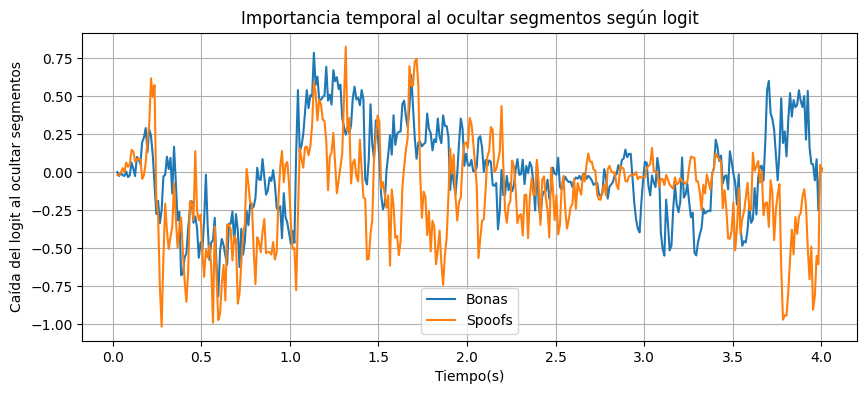
\includegraphics[width=\textwidth]{imagenes/AASIST_global_occlusion_temp_logit.png}
	\caption{Resultados de ``logit'' de la ocultación temporal en AASIST.}
\end{figure}

En esta primera gráfica, vemos como ayuda cada tramo a los logits de los audios de cada clase. En lo referido a la clase ``bona'', podemos destacar tres fases: 
\begin{itemize}
    \item Entre \textbf{0,3 y 0,9} segundos, donde predominan valores negativos, es decir, no aporta evidencia útil al logit de la clase e incluso podría introducir información ambigua.
    \item Entre \textbf{1,0 y 1,8} segundos, donde se encuentran valores muy por encima del resto de la gráfica. Podemos deducir que es la zona donde el modelo encuentra más información importante para la clasificación de esta clase.
    \item Entre \textbf{3,7 y 3,95} segundos, vuelve a aparecer una región claramente positiva. Sin embargo, como rellenamos los audios más cortos hasta 4 segundos, esta última franja puede estar parcialmente contaminada.
\end{itemize}

Sobre la clase ``spoof'', tenemos una gráfica bastante distinta con 4 regiones:
\begin{itemize}
    \item Entre \textbf{0,15 y 0,3} segundos, un pico positivo muy superior al resto de la zona.
    \item Entre \textbf{0,3 y 1,0} segundos, al igual que con la clase ``bona'', una zona con valores claramente negativos que indican la misma conclusión.
    \item Entre \textbf{1,2-1,4 y 1,5-1,8} segundos, volvemos a ver picos positivos que empujan el logit hacia la clase ``spoof''.
    \item Entre \textbf{3,8 y 4,0} segundos, una región negativa claramente diferenciada. Sin embargo, la precaución explicada para la clase ``bona'' también se aplica aquí.
\end{itemize}

En resumen, esta gráfica sugiere que el modelo se apoya en tramos concretos y no en toda la señal. En la clase ``bona'', la evidencia está muy localizada en la zona central, mientras que la clase ``spoof'' usa evidencia spoof menos estable y, seguramente más basada en patrones o irregularidades locales.

\begin{figure}[H]
    \centering
	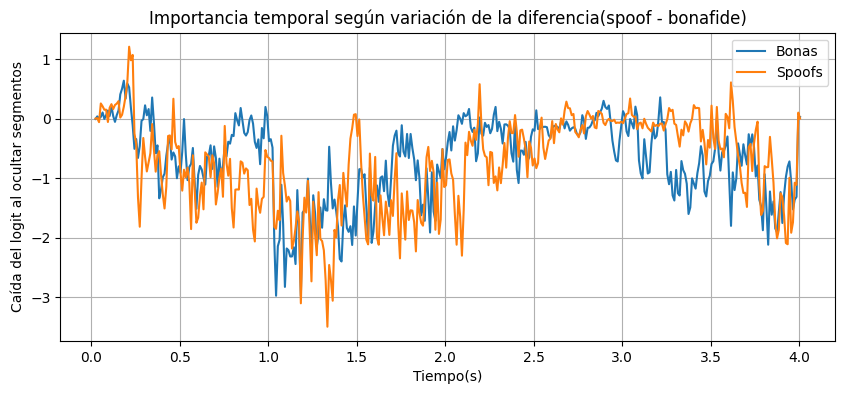
\includegraphics[width=\textwidth]{imagenes/AASIST_global_occlusion_temp_margin.png}
	\caption{Resultados de margen de la ocultación temporal en AASIST.}
\end{figure}

Para interpretar esta gráfica, conviene recordar que al mostrar la variación del margen entre clases, las zonas positivas son segmentos \textbf{pro-spoof} y las negativas, \textbf{pro-bona}. Esta aclaración se aplica para ambas curvas, ya que para ambos casos calculamos el margen como la diferencia entre la salida de la clase ``spoof'' y la de la clase ``bona''.

En cuanto a las regiones más relevantes, podemos señalar dos: la comprendida entre \textbf{0,2 y 0,3}, la cual es pro-spoof, especialmente la curva ``spoof''. Esto signfica que el modelo encuentra evidencia que le empuja la decisión hacia ``spoof''. La segunda región que se encuentra entre \textbf{1,0 y 2,0} segundos, la cual empuja la decisión claramente a ``bona''. 
Sobre el patrón general de la gráfica, podemos intuir que los audios ``spoof'' parecen naturales la mayor parte del tiempo ya que la mayoría de valores son negativos. Sin embargo, AASIST debe encontrar patrones muy localizados que le ayudan a clasificar los audios como spoof.

\begin{figure}[H]
    \centering
	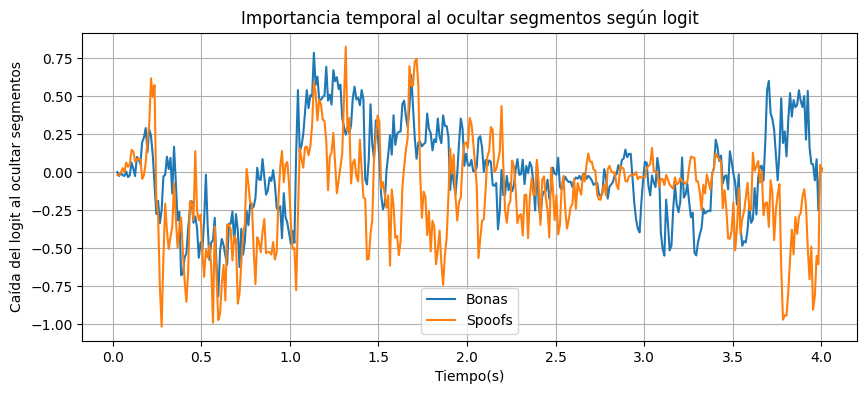
\includegraphics[width=\textwidth]{imagenes/AASIST_global_occlusion_frec_logit.png}
	\caption{Resultados de ``logit'' de la ocultación temporal en AASIST.}
\end{figure}

En la gráfica, podemos observar claramente como la banda 0-500 Hz es muy dominante, e incluso, el tramo 500-1000 Hz en ``bonas''. Esto es coherente con lo que uno espera de la voz humana, ya que en las bajas frecuencias se concentra no solo la frecuencia fundamental, habitualmente situada en torno a 80-300 Hz, sino también una parte importante de la energía global de la señal y de su estructura armónica.

Asimismo, es importante mencionar, que aunque ambas curvas tienen comportamientos bastantes planos en general, esto puede no significar que sean poco relevantes. Es posible que contengan información repetida de forma redundante en otras bandas.

\begin{figure}[H]
    \centering
	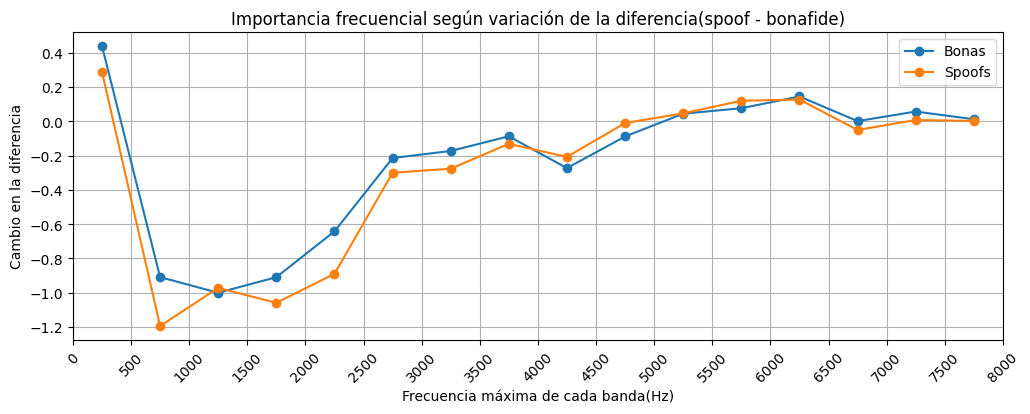
\includegraphics[width=\textwidth]{imagenes/AASIST_global_occlusion_frec_margin.png}
	\caption{Resultados de margen de la ocultación temporal en AASIST.}
\end{figure}

En esta gráfica podemos destacar tres regiones:
\begin{itemize}
    \item Tramo \textbf{0-500} Hz: en esta banda hay valores positivos lo que significa que favorece el margen hacia spoof. Aunque pueda parecer contradictorio con la gráfica anterior, una banda puede ser importante para una clase pero, sin embargo, al considerar el margen, favorecer más a la clase contraria.
    \item Tramo \textbf{500-2000} Hz: aquí encontramos curvas negativas, es decir, es una región pro-bona. Esto puede tener sentido ya que estas frecuencias se consideran muy importantes para la inteligibilidad del habla. 
    \item Tramo \textbf{5500-6500} Hz: aparece una contribución ligeramente positiva. Esto podría estar relacionado con algun patrón artificial de altas frecuencias.
\end{itemize}

\begin{figure}[H]
    \centering
    \begin{subfigure}[t]{0.49\textwidth}
        \centering
        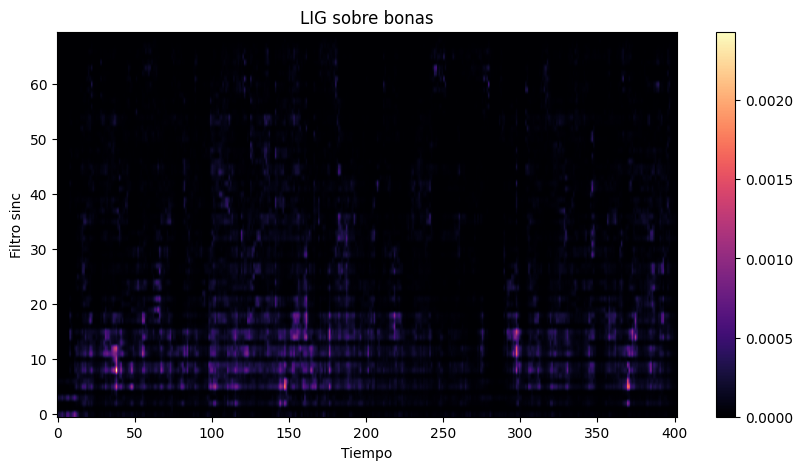
\includegraphics[width=\linewidth]{imagenes/AASIST_global_LIG_bonas.png}
        \caption{Mapa filtro-tiempo generado con IG para ``bonas''.}
        \end{subfigure}
    \hfill
    \begin{subfigure}[t]{0.49\textwidth}
        \centering
        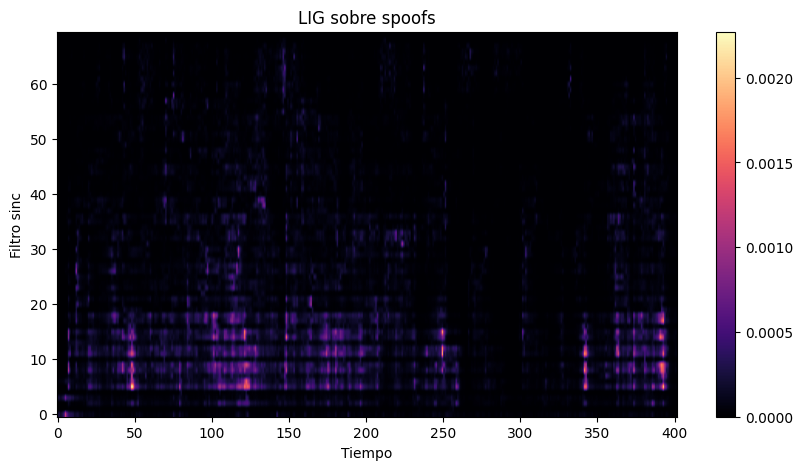
\includegraphics[width=\linewidth]{imagenes/AASIST_global_LIG_spoofs.png}
        \caption{Mapa filtro-tiempo normalizado generado con IG para ``spoofs''.}
    \end{subfigure}
\end{figure}

Lo primero destacable, es que aquí, mostramos la magnitud absoluta de atribución, no signo, por lo que solo podemos destacar relevancia espectral pero no si una región empuja a cierta clase.

Interpretando los comportamientos, por un lado, observamos actividad predominantemente focalizada en los filtros bajos en el mapa de ``bonas''. Por otro lado, en el mapa de ``spoofs'', aunque también observamos esta predominancia, aunque se observa una actividad algo mayor en las frecuencias altas. Esto podría reforzar la idea mencionada de patrones artificiales o irregularidades espectrales en frecuencias superiores.

\begin{figure}[H]
    \centering
    \begin{subfigure}[t]{0.49\textwidth}
        \centering
        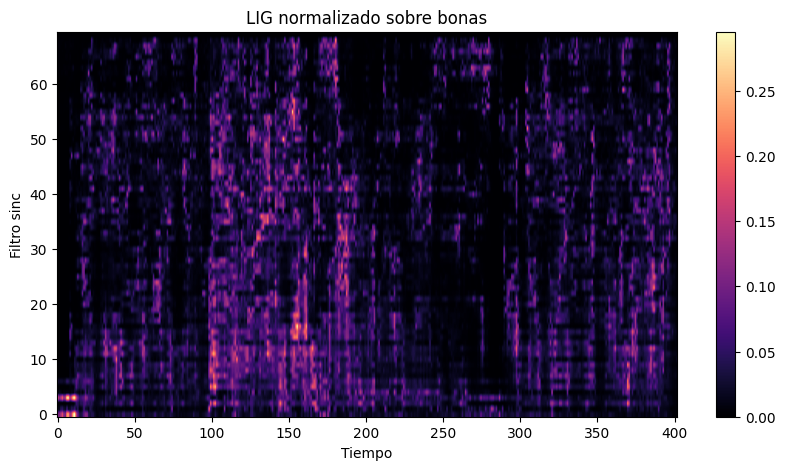
\includegraphics[width=\linewidth]{imagenes/AASIST_global_LIG_bonas_norm.png}
        \caption{Mapa filtro-tiempo generado con IG para ``bonas''.}
        \end{subfigure}
    \hfill
    \begin{subfigure}[t]{0.49\textwidth}
        \centering
        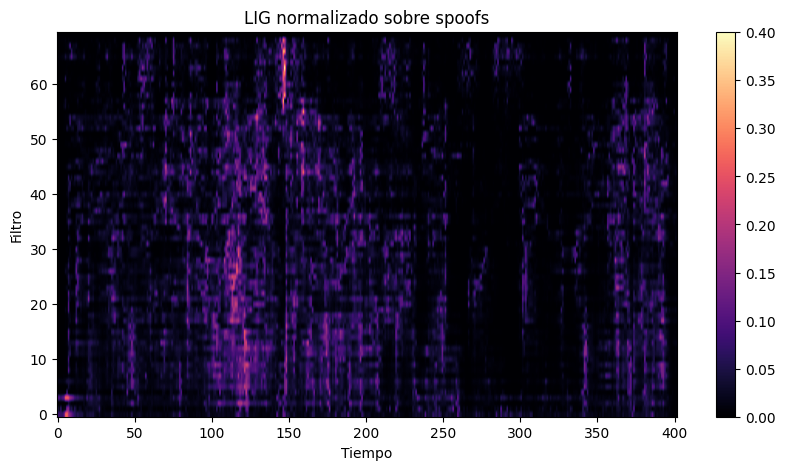
\includegraphics[width=\linewidth]{imagenes/AASIST_global_LIG_spoofs_norm.png}
        \caption{Mapa filtro-tiempo normalizado generado con IG para ``spoofs''.}
    \end{subfigure}
\end{figure}

Los mapas normalizados explican mejor como se reparte la importancia entre filtros y a lo largo del tiempo al reducir el efecto de las bandas con mayor magnitud absoluta.

En ambas gráficas, seguimos obsevando actividad casi continua de los filtros bajos en los 4 segundos. Respecto al mapa de ``bonas'', destaca la región entre \textbf{1 y 2} segundos donde hay más actividad. Esto coincide con lo mencionada en la gráfica temporal con ``logits'' de Occlusión. 

En el mapa de ``spoofs'', vemos una actividad más fragmentada y localizada en eventos temporales concretos, como por ejemplo entre los segundos \textbf{1 y 1,5}, y entre los segundos \textbf{3,6 y 3,9}. Ambas regiones también coinciden con las deducciones sacadas en Occlusion temporal.

\begin{figure}[H]
    \centering
	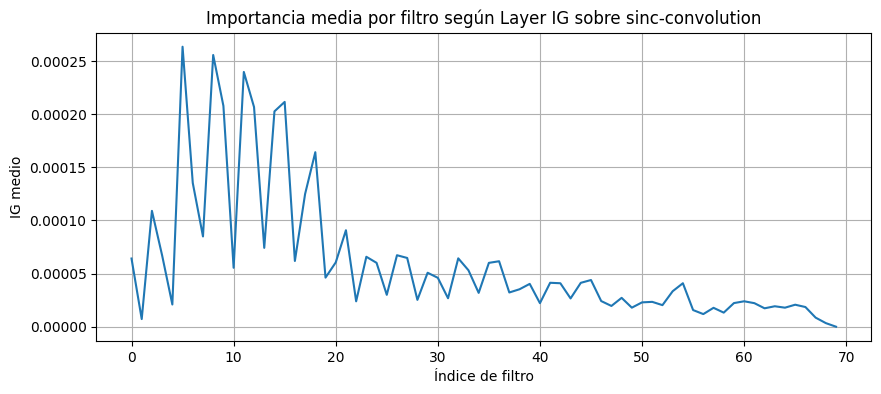
\includegraphics[width=\textwidth]{imagenes/AASIST_global_LIG_grafica.png}
	\caption{Gráfica filtro-tiempo de la capa sinc-convolution.}
\end{figure}

Esta gráfica aporta información más detallada sobre las bandas de frecuencias bajas, nos señala con mayor precisión, dentro de este conjunto, cuales son los más excitados. En particular, se observan varios picos destacados entre los filtros 5 y 20, lo que sugiere que la contribución del modelo no se distribuye de forma uniforme entre todos los filtros bajos.